\documentclass[conference]{IEEEtran}
\IEEEoverridecommandlockouts
% The preceding line is only needed to identify funding in the first footnote. If that is unneeded, please comment it out.
\usepackage{cite}
\usepackage{amsmath,amssymb,amsfonts}
\usepackage{algorithmic}
\usepackage{graphicx}
\usepackage{textcomp}
\usepackage{xcolor}
\def\BibTeX{{\rm B\kern-.05em{\sc i\kern-.025em b}\kern-.08em
    T\kern-.1667em\lower.7ex\hbox{E}\kern-.125emX}}
\begin{document}

\title{Term Project Part-2\\
{\footnotesize }
}

\author{\IEEEauthorblockN{Abdullah Mert Tuncay}
\IEEEauthorblockA{\textit{Departmen of Computer Engineering} \\
\textit{Middle East Technical University}\\
Ankara, Turkey \\
2099422 \\
e2099422@ceng.metu.edu.tr}
\and
\IEEEauthorblockN{Baris Sugur}
\IEEEauthorblockA{\textit{Departmen of Computer Engineering} \\
\textit{Middle East Technical University}\\
Ankara, Turkey \\
2099315 \\
e2099315@ceng.metu.edu.tr}
}

\maketitle


\section{Introduction}
According to given topology from the Term Project Part 2, we designed a simple network which consists of 5 different nodes. In this document, we will start with the explanation of our design and how we implemented it. Then, we will share our experimental results about the implementation to show how our reliable network behave in different manners. At the end, we share our experiences and comments about these parts of the projects.

\section{Design Approach}

\subsection{Understanding of the Topology}

According to the given topology, we are given 5 different nodes to construct a network. Each node has its own tasks which will be decided accordingly our design. Starting with the source node, we stated that node as our client node and destination node as our server node. After that, we went on to the other nodes which are broker and routers. These nodes have individually different tasks since they have links to the both client and server sides. Starting with the broker, it has the most special tasks in design because it is acting like a converter in TCP and UDP part of the project. As stated in the topology we have a link which uses TCP between source and broker. On the other side, links between broker-routers and routers-destination uses UDP connection. Since broker has links for both sides, it needs to include sockets for both sides. Also, we do not implement any socket programming for routers in this part of the project. Since their task is simply forwarding one interface to another interface.

\subsection{Socket Programming Part}

After understanding how the nodes reacting each other, we focused on how we construct this links in our design. We simply meet socket programming which is the main approach for constructing this type of networks. According to socket programming, we have two type of nodes client and server. But in our topology as I mentioned above, we have different nodes which acting like both. In source node, we have client which initiates the connection. According to socket programming, client needs to now the address and the port of the server which will be the node that receives data or message. It's socket named as active socket. While moving onto the other nodes, we think other nodes as both client and server node(excluding the destination node) because these nodes both initiates the connection and wait  and respond for the clients. With this thought, we opens two sockets for the broker node. One node uses a socket with TCP connection to wait and respond the requests from the source node. On the other hand, second node uses 2 sockets with UDP connection to connect r1 and r2 routers. At the end, r1-destination and r2-destination uses UDP sockets,too.

\subsection{TCP vs UDP Sockets}
While designing the TCP and UDP sockets, we acknowledge some differences and we follow and implement according to it.In TCP, when a TCP client send data to the server, it requires an acknowledgement in return. If an acknowledgement is not received, TCP automatically retransmit the data and waits for a longer period of time. In UDP, the client does not establish a connection with the server. Instead, the client just sends a datagram to the server with requiring the address of the destination. Similarly, the server does not accept a connection from a client. Instead, the server just waits until data arrives from some client. At the end, the IP address of the client and the datagram is received, so the server can send a response to the client using these. But according to researches, UDP datagrams are characterized by a length while TCP is a byte-stream protocol, which do not have any boundaries. 

\subsection{RDT in UDP and Go-Back-N}
After understanding TCP and UDP properties, we are expected to implement a Reliable Data Transfer for UDP part of the topology. Since UDP just waits until the data arrives and do not notify the client which is broker in this case. We needed to implement an algorithm which sends some acknowledgement to notify related to the received packet. This gives us a reliable data transfer property in UDP. We used Go-Back-N system for this acknowledgement part. Thanks to this system, we can easily managed to request the re-transmission of the missing packets and packets with errors. Since packets can be arrive in different order or after the timeout time, with this approach we are able to refresh our packets. While checking the packets correctness we using a checksum variable which is defined for our UDP transfer. Also we have an expected packet number variable which is increasing one by one according to arriving packets. If the arriving packet number is wrong, we return to the last successively received packet number. So, we used retransmission, checksum , ack/nack principle and expected packet number(sequence number) for our RDT implementation.

\subsection{Multihoming and Pipelining}
In out task, we need to use RDT on both routers and make broker a multihoming node. With threads, we are expecting to implement a multihoming network. Also we need our network to work in a pipelining principle. So using threads we are sending packets over two different threads which are using two different routers.

\subsection{Message in TCP and UDP}

As a message, we used 5MB input file which was given to us. We send this file differently in TCP and UDP. In TCP, we send as packets of 1024 bytes. In UDP part, we divide this data into 900 bytes. Because our packet has also consist header part which is approximately 100 bytes. So if we add up this parts, our packet is about 1000 bytes. In our implementation, we are calculating the message length by using len function in the python.


\section{Implementation Approach}

\subsection{Geni Platform and Programming Languages Choice}

At the beginning, we download the topology XML file to add resources in Geni platform. Then we use MAXI Insta Geni resources to go with. Then, we think about choosing Python which has an simple approach for handling socket programming. We examined the Python libraries according to our use and decided to choose it for our term project.
\subsection{General Features for Nodes}

For all node, there are several things that we do the same. Since we are using sockets to establish a connection between nodes, we kept HOST and PORT for the nodes. Excluding source nodes, all of our nodes consist multiple sockets since they have multiple links. At the broker node, we have 3 different sockets. One TCP socket for source node and 2 UDP socket for r1 and r2. Also, we use different ports for r1 and r2. For r1 and r2 node, we have directed the sockets between the destination and the broker. We use two different shell-scripts for this matter in router1 and router2. This shell-scripts are using \textbf{sudo route add -host IP-address interface-for-coming gw interface-for-going} terminal command to direct the packets from one to another IP address. At the end, for destination node we have 2 sockets which connects to broker using r1 and r2. In addition to these, we also construct a infinite loop to receive message .
\subsection{TCP Socket Implementation}

We construct a base client and server implementation for our TCP connection between source and broker. We opening a TCP socket with socket() function. Its parameters define the address family and socket type. Since TCP sends stream of data the term SOCK STREAM symbolize it. Also "AF INET" is Internet address family for IPv4. Then we connect the socket to server with server's hostname and port number used by the server. We are reading the input file by 1024 bytes and sending 1024 bytes by using sendall() while there is a input message. At the server side, after we defining the socket, we bind the socket and make it listen to port until a connection received. Then we started a while loop, then accepted connection. From this connection, we received data by 1024 bytes and writing this data to an output file. After TCP connection received all the 5MB data from the source node, we start to send data over UDP links.

\subsection{Broker Implemtation}

In broker implementation, we are having 1 TCP socket and 2 UDP sockets. After the definition of the HOST and PORT(which is the same for all nodes), we constructing a two sending sockets. These sockets are used to make a link between the routers and broker. After the UDP sockets are defined, we are constructing our TCP sockets to receive data. In this part, broker act like a server and bind to HOST and PORT and starting to listen to sockets for upcoming connection. Then inside an infinite loop, the connection was made and using the connection we received the data. This infinite loop also terminate if the data is not received after the connection.

\subsubsection{Broker Thread Implementation}

Currently we are using two threads for our broker implementation. One thread is sending data over router1 and the other one is sending data over router2. While creating threads, we use threading.Thread function for each thread. Their parameters are the sending message function as target and functions arguments as args. In args, first one is message until the first part ends which is exactly the half of the message length for the first thread and all message length for the second thread since we are using 2 threads and the second one is message offset which is the starting byte number in our message which is 0 for our first thread and half of the message for the second thread. This two threads are using different routers.


\subsubsection{Broker Sending Data Implementation}

Since we are using threads for the broker sending data, we have function as we mentioned which have arguments message length and message offset. We have two different arrays for broker addresses and destination addresses. This two arrays consists the IP addresses for the links that connects the broker and destination over router1 and router2. After that we constructed a variable for maximum message segment size. We choose this variable as 900. Because our boundary for the packet is 1000 byte and we think that our header is approximately 100 bytes. So we choose to read packets of size 900. After that we constructed a window size variable which is 5 for checking Go-back-N system. So we send 5 packets before ACK received and check whether their correctness. Also there is unique checksum number for reliability. We also initialized a variable which input message for usages in the read part. After that we are converting the coming inputs to integers since they are coming as a output of division operation. Then we initialize variables close,closer counter and go back N for their named usages. Close is for notifying that the message is finished. Closer counter is used to close connection for any problem. go back N variable used for the waiting ACKs. After that we are reaching the current threads and uses its number to decide which link and port will be used. We decide the address of the broker as well. After that constructed a UDP socket and bind it to the current broker address. We also initialize packet number as 0 which is incremented by every iteration. Then we started a while loop while the message offset is less than message length. In this while we are reading the input data as a 900 bytes parts. At the begging of the while loop, we are checking whether we are reached the end of the data or not. Then we are using to hash algorithm with md5(). After that message and checksum turning into string and concatenating. Updating the check sum variable with byte version of this string. After these parts, we are generating the message header. Our message header includes Current broker address, Current destination address,Packet number,Check sum and close flag. After that we serialize the message segment which consists message header and message part. We are serializing this message to sent over UDP send to function. In this serialization, we are using marshal other than pickle or cPickle for being fast. But if we want to change our serialization is to pickle or cPickle, we only need to change marshal part to pickle or cPickle.
After sending the message segment, we are incrementing the go back N variable by one. Since we sent the message, now we are checking whether the go back N variable reaches the window size 5 for RDT. If we did not send the data in order, message ack not receive until the timeout occurs or some message packet lost, we will send these five packets according to the given ACK. Also there is an another elif statement which stands for whether the end of file is reached or not. After this while ends, we are closing the sockets of UDP. 


\subsection{Destination Implementation}

In destination, we implemented threading as well and using os.system properities, we are creating two different files for two different data coming from two different paths. At the end, we are uniting this two different files and delete these files. About the receive message part, we are receiving the messages. After that we are separating the header from the received message segment. Checking whether receiving message packet is correct and sending acknowledgement related to it.
\subsubsection{Destination Thread Implementation}

In this part we are using two thread as well to receive data from two different connections which comes from two different routers. So as a target in threading function, we are giving receive message function to work on the chosen thread. we are appending this threads and starting iteratively. After that we are joining them.
\subsubsection{Destination Receive Data Implementation}

We are initializing an expected packet number as 0 and accessing the current thread. By using current thread, we are setting up the connection and opening a new file to write the upcoming data. After that we are using an infinite loop to receive the data and send acknowledgements. At the beginning we are incrementing the expected packet number by 1. After that we are receiving the packet of 1000 bytes and deserializing it using marshal loads function. We are dividing this message into broker data header and main message. This broker data header consists broker address, message packet number and message checksum. Then we are using hashlib to construct expected checksum number. At the end of this file parsing, we are starting to check whether the data is receive correctly. First, we are checking whether the checksum number and the expected checksum number is matched. Since we need to check whether this data coming from the expected links or not. If not, we are sending the last received successful message packet number as ACK which is expected message number minus 1 and decreasing the expected message packet number. So if the checksum is matched, we are checking whether the message packet number is equal to the expected packet number. So this tells us that may be the order is wrong or a packet is missing. If we are not able to receive the data in correct order, then we are sending the expected message number minus 1 and decreasing the expected message packet number again. If all of this parts can be passed, we are sending the message packet number as ACK we tells broker that the packet is received successfully. Not that in all parts that we are sending ACK, we are using marshal serializing before sending the ACK. At the end if the close flag is set, we are breaking from the infinite loop and this ended up with the close of socket. 

\subsection{UDP Socket Implementation}

In the broker, we initialize our first UDP sockets. The term SOCK DGRAM is telling us about the sockets that this socket will use UDP connection. We defined 2 send sockets for our 2 different routers r1 and r2. Then send the data according to the message lengths. The operation in r1 and r2 is about transmitting the data between them. After receiving data and sending it to the destination by using sendto(), we are receiving these datas in destination by using two different routers by using two different threads. In these UDP links, we do not ever need to make a connection or listen to it. We just bind to the related host and port and wait for receiving the data. After the data which is coming from r1 and r2, we are making some calculations and sending acknowledgement back to the broker. 


\subsection{End-to-End Delay Calculation}

Since there is a TCP connection between source and broker, we used this connection to send the file directly, so the delay part we calculated is summation of time past between source-broker and broker-destination. The time between source and broker is much lower (as expected) than time passed between broker and destination. For source-broker transmission, it takes around 20 seconds for the file to transfer. And without any packet loss or error, it takes approximately 90 second for 5MB file to reach the destination from broker. (Note that this time is higher for packet loss configurations because some packets are retransmitted, but time between source and broker stays same) Detailed graphs and end-to-end time according to these packet losses are given below. 

\section{Experimental Results}

Below there are 3 bar graphs that includes 3 different experiment. These experiments were generated by using the commands that was provided to us. So we included the graphs that added loss, corruption and reordering the our reliable networks respectively and independently.


\subsection{Packet Loss}

Below is the graph that sends the message with packet loss of 0.5, 10 and 20 respectively. From this graph, we will see that the results when the packet loss is applied.

\begin{figure}[h]
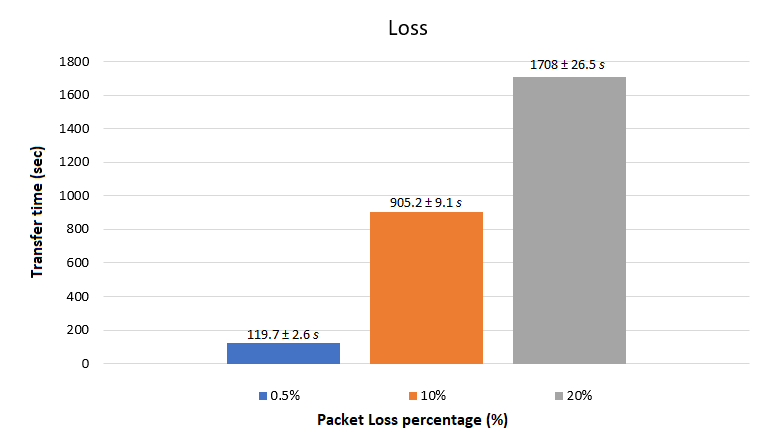
\includegraphics[width=0.45\textwidth]{Loss.png}
\caption{Loss Experiment}
\label{fig:figure2}
\end{figure}


The packet losses and their related number shown in the below table respectively : \\


\begin{tabular}{||c | c | c | c ||} 
  \hline
  Packet Loss & \%0.5 & \%10 & \%20  \\ [0.5ex] 
  \hline\hline
 Sample Size  &  9  & 6  & 4 \\ 
 \hline
 Mean         & 119.7 & 905.2 & 1708  \\ 
 \hline
 Standard Deviation &  4 & 11.3 & 33.2  \\ 
 \hline
  Mean*\%2.5         & 2.99 & 22.6 & 42.7  \\ 
 \hline
\end{tabular}
$\vspace*{0.4in}$\\

For this graph, both our connection and nodes connections was a bit ambiguous, so the graph didn't turned out to be a perfect but it still make sense. The \%95 confidence interval can be calculated with the following formula:

$$X \pm Z \dfrac{s}{\sqrt{n}}$$
Where; \\
X = mean \\
Z = 1.96 (for \%95 confidence interval) \\
s = standard deviation \\
n = sample size \\
Hence, for this graph, the confidence interval for the three experiment in packet loss can be calculated :\\

For packet loss with \%0.5:
$$119.7 \pm 1.96 \dfrac{4}{\sqrt{9}} = 119.7 \pm 2.6s$$
For packet loss with \%10:
$$905.2 \pm 1.96 \dfrac{11.3}{\sqrt{6}} = 905.2 \pm 9.1s$$
For packet loss with \%20:
$$1708 \pm 1.96 \dfrac{33.2}{\sqrt{4}} = 1708 \pm 26.5s$$

From the above calculation you can see that the resulting values are less than the their respected values in the table which is Mean*\%2.5.

As from the above calculations and the results, we clearly see that the packet loss simulations is incremented the time while the packet loss percentage is increased. We also see that the resulting values from the standard deviations are calculated less than the needed values.

\subsection{Corruption}

Below is the graph that sends the message with corruption parameter with \%0.2, \%10 and \%20 respectively. From this graph, we will compare the end-to-end time change when the corruption simulation is applied.

\begin{figure}[h]
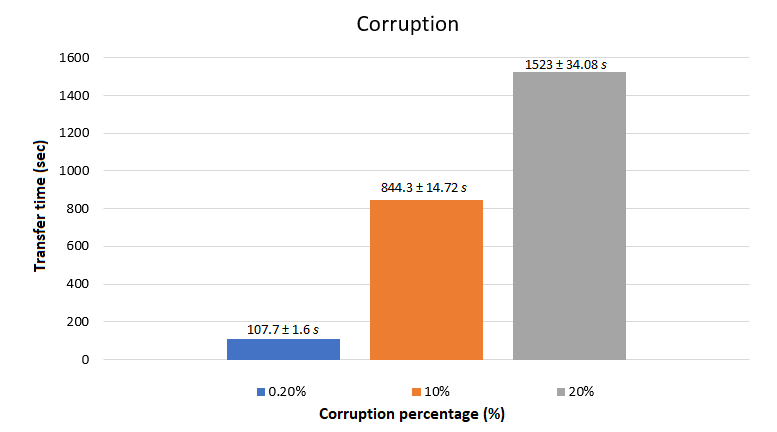
\includegraphics[width=0.45\textwidth]{Corruption.png}
\caption{Corruption Experiment}
\label{fig:figure2}
\end{figure}

Corruption and their related number shown in the below table respectively : \\

\begin{tabular}{||c | c | c | c ||} 
  \hline
  Corruption & \%0.2 & \%10 & \%20  \\ [0.5ex] 
  \hline\hline
 Sample Size  &  9  & 6  & 6 \\ 
 \hline
 Mean         & 107.7 & 844.3 & 1523  \\ 
 \hline
 Standard Deviation &  2.4 & 18.4 & 42.6  \\ 
 \hline
 Mean*\%2.5         & 2.69 & 21.1 & 38.1  \\ 
 \hline
\end{tabular}
$\vspace*{0.4in}$\\

For this graph, the confidence interval for the three experiment with corruption can be calculated :\\

For corruption with \% 0.5:
$$107.7 \pm 1.96 \dfrac{2.4}{\sqrt{9}} = 119.7 \pm 1.6s$$
For corruption with \%10:
$$844.3 \pm 1.96 \dfrac{18.4}{\sqrt{6}} = 844.3\pm 14.72s$$
For corruption with \%20:
$$1523 \pm 1.96 \dfrac{42.6}{\sqrt{6}} = 1523 \pm 34.08s$$


From the above calculation you can see that the resulting values are less than the their respected values in the table which is Mean*\%2.5. \\


As from the above calculations and the results, we clearly see that the corruption simulations is incremented the time while the corruption percentage is increased. We also see that the resulting values from the standard deviations are calculated less than the needed values.

\subsection{Reorder}

Below is the graph that sends the message with reordering parameter \%1, \%10 and \%35 respectively. From this graph, we will compare the end-to-end time change when the reordering simulation is applied.

\begin{figure}[h]
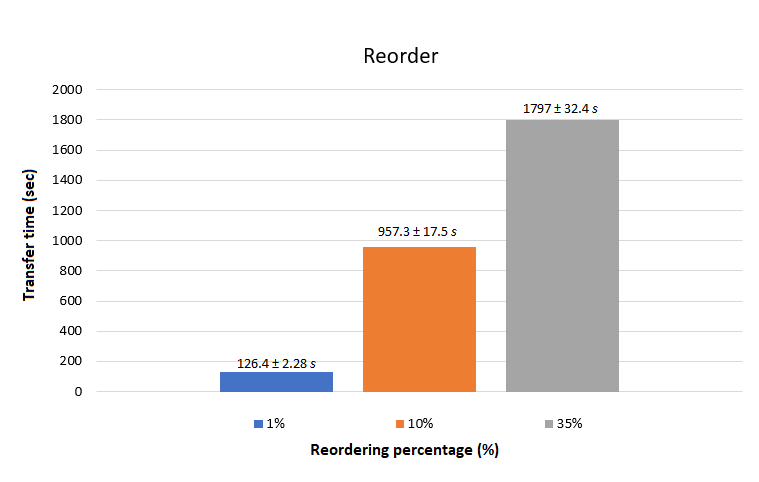
\includegraphics[width=0.45\textwidth]{Reorder.png}
\caption{Reorder Experiment}
\label{fig:figure2}
\end{figure}

Corruption and their related number shown in the below table respectively : \\

\begin{tabular}{||c | c | c | c ||} 
  \hline
  Reorder & \%1 & \%10 & \%35  \\ [0.5ex] 
  \hline\hline
 Sample Size  &  8  & 6  & 4 \\ 
 \hline
 Mean         & 126.4 & 957.3 & 1797  \\ 
 \hline
 Standard Deviation &  4.1 & 21.9 & 33.1  \\ 
 \hline
  Mean*\%2.5         & 3.16 & 23.9 & 44.9  \\ 
 \hline
\end{tabular}
$\vspace*{0.4in}$\\



For this graph, the confidence interval for the three experiment with corruption can be calculated :\\

For corruption with \% 1:
$$126.4 \pm 1.96 \dfrac{4.1}{\sqrt{8}} = 126.4 \pm 2.28s$$
For corruption with \%10:
$$957.3 \pm 1.96 \dfrac{21.9}{\sqrt{6}} = 57.3 \pm 17.5s$$
For corruption with \%35:
$$1797 \pm 1.96 \dfrac{33.1}{\sqrt{4}} = 1797 \pm 34.08s$$

From the above calculation you can see that the resulting values are less than the their respected values in the table which is Mean*\%2.5.\\


As from the above calculations and the results, we clearly see that the reordering simulations is incremented the time while the reordering percentage is increased. We also see that the resulting values from the standard deviations are calculated less than the needed values.

\section*{Comments}

\subsection*{}
In the part-2 of the term-project, we happen to encounter many of the different problems and errors. Many of the related issues are about the serialization techniques we used and the size of the packets. Since we need to calculate the most suitable packet size for the sending packet.

\subsection*{}
In the design part, we start to think as simple as possible to prevent complicated errors while constructing the topology we are given. After the simple implementation is finished, we focused on the main task about how we can change to do better or how we can do it faster. We wrote a script that changes all files in the nodes with the local ones. On the other hand, we focus on the message part first about how we can customize it to our needs. This shows us the difference between the message length or size limit difference in UDP and TCP. 

\subsection*{}

While implementing the Reliable Data transfer, we need to think about some possibilities like corruption, reordering and packet loss as we guided to check when finished. Since their implementation need some different algorithms but mostly their algorithms completed each other. But while implementing reliable network, we need to move step-by-step. We first implemented the socket connection between the destination and broker part. After that we started to implement the parts for how we check the correct message packet is received. For this usage, we used Go-back-N and checksum properties. We use a not much but reasonable size for our window size using in the Go-back-N algorithm. But the test part is have some difficulties related to some miss if-else statement usage. After we corrected these parts, our program can easily receive and checking the messages.

After the acknowledge receive part was implemented, we added some timeout and exception proprieties for save usages in our design. In this part, we are able to test the windows sending by decreasing the timeout to very small values, so we are able to check whether the parts are completed correctly or not. 

With all the parts we implemented, connection related to nodes and the file sending is some small but important issues that we faced. We handled these by writing some python scripts to simplify our tasks in this.

\section*{Workload over Team Members}

\subsection*{}

As a team, we wrote the coding part as a team. We worked simultaneously. We tried our own solution while working together and updated our code according to the best solution. In the reporting part, we opened a project on the overleaf website and edited the latex file simultaneously. While one member were writing a subsection the other one completed the other subsection and controlled each others part. After that, we moved on the next subsection. In the experiment part, we did experiments by using Baris's computer which is more stable than Mert's. After collected the result of the one experiment, the other one did the necessary calculations related to it and again we checked each others work after finished.  

\end{document}
